\documentclass[10pt,twocolumn]{article}
\usepackage{fullpage,enumerate,amsmath,amssymb,graphicx,setspace,epstopdf,float,multirow}

\begin{document}
\title{CS 276 Programming Assignment 2 Project Report}
\author{Jiaji Hu, Xuening Liu}
\date{}
\maketitle
\section{System Design}
\subsection{Code Structure}
\texttt{BuildModels} and \texttt{RunCorrector} are used to build models and run the spell corrector, respectively.

\texttt{LanguageModel} and \texttt{NoisyChannelModel} builds the language and noisy channel models during model building time, which are saved to disk and loaded when needed in the future.

\texttt{EditCostModel} is the interface, while \texttt{UniformCostModel} and \texttt{EmpiricalCostModel} are the cost models used to compute edit probabilities.
\subsection{Model Building}
\subsubsection{Language Model}
To building the language model, we go through the training corpus, building up our unigram and bigram dictionaries. For alternative smoothing methods, we also need to document the number of unique bigram continuations and number of possible following words.

To conform with memory requirements and still save the information for the extra credit, we implemented a \texttt{Triple} class and a \texttt{TriDictionary} class to store entries.
\subsubsection{Noisy Channel Model}
To build the noisy channel model, we go through the training edit file, collect 3 kinds of statistics: count of single character, count of pair characters and count of errors to train the model. For count of error, we defined a new class \texttt{Error} to store the error type, and error string.

\subsection{Error Correction}
At query time, the input query is fed into the candidate generator to generate candidates with edit distance lesser or equal to 2. The candidate generation process is discussed in detail in Section 2.

After this, we want to calculate $P(Q|R)$, where R is the actual input, and Q is the candidate. We know $P(Q|R)\propto P(Q)P(R|Q)$, where $P(Q)$ is calculated with the language model, and $P(R|Q)$ is calculated using the noisy channel model. For scoring, we use $P(Q|R)\propto P(Q)^\mu P(R|Q)$, where $\mu$ is a parameter we tune for performance.

For the language model, $P(Q)=P(w_1,\dots,w_n)=P(w_1)P(w_2|w_1)\dots P(w_n|w_{n-1})$. We use maximum likelihood estimation for these unigram and bigram probabilities, with smoothing for the bigram probabilities. Smoothing methods are discussed in depth in Section 3.

For the noisy channel model, if we are using uniform edit probabilities, then we simply assume that any edit of edit distance one occurs with the same small probability. If we are using the empirical cost model, we first detect the error type, which is used to find corresponding statistics collected during training to calculate error probabilities.
\section{Candidate Generation}
To generate candidates of edit distance 1, we created a method \texttt{editDistanceOne()} based on Peter Norvig's approach. To generate distance 2 candidates, we run \texttt{editDistanceOne()} on the distance 1 results. After computing candidate words, we compare them to the dictionary to filter out invalid ones so that we don't have to score them.
 
There is an obvious tradeoff regarding candidate generation. On one hand, if the right answer was not even generated, the output query cannot be correct, so we want to cover as much space as possible. On the other hand, generating and scoring large amounts of candidates uses excessive runtime and memory.

With this tradeoff in mind, we looked at three strategies for generating distance 2 candidates, in the order of increasing number of candidates generated: (note that we define an output of the generator to be a ``raw" candidate, and a raw candidate to be ``valid'' if all its words appear in the unigram dictionary.)

1. Only generate distance 2 candidates if there is no valid distance 1 candidate.

2. Generate distance 2 candidates from all {\it valid} distance 1 candidates.

3. Generate {\it all} distance 2 candidates.

\begin{table}[ht]
\begin{tabular}{| c | c | c | c | c |}
\hline
Strat. & Time & Valid cand. & Raw cand. & Accur.\\\hline
1 & 10 & 50,000 & few & 86.1\%\\\hline
2 & 50 & 5,600,000 & many & 88.5\%\\\hline
3 & 150 & 5,800,000 & {\it very} many & 90.0\%\\\hline
\end{tabular}
\end{table}

As shown above, the tradeoffs are quite obvious. By optimizing our code (including a novel optimization where we avoid repeat generation of any raw candidate by ordering our generation steps - its complicated), we were able to cut down on runtimes, so that we could get away with generating vast amounts of raw candidates. By filtering raw candidates with our dictionary, we make sure not to score useless candidates. If runtime becomes an issue, we can always fall back on a faster, but slightly less accurate strategy.
\section{Methods}
\subsection{Smoothing for Edit Probabilities}
To assign probabilities for edits that are not found in the training edit file, we first used simple add-one smoothing. To try to improve on that, we switched to add-delta smoothing, and tested some values of delta. The value of delta did not do much to improve accuracy.

\subsection{Smoothing for Language Model}
\subsubsection{Original method (Jelinek-Mercer)}
Smoothing is done to try to account for the data sparsity problem. If a query had a bigram that was not seen during training, we don't want its probability to be zero.

The assignment instructions suggest we interpolate unigram probabilities with bigram probabilities to get the final conditional probability like so:
\begin{equation*}
P_{int}(w_2|w_1) = \lambda P_{mle}(w_2) + (1-\lambda)P_{mle}(w_2|w_1)
\end{equation*}
In practice this smoothing method gives good results. However, we can still explore other possibilities.
\subsubsection{Katz (back-off) method}
When trying to estimate $P(w_2|w_1)$, the backoff model\cite{katz1987estimation} uses $P_{mle}(w_2|w_1)$ if $count<w_2,w_1>$ is larger than some threshold (e.g. 0). Else, the model backs off to use $P_{mle}(w_2)$. This also works with weights. In doing this, the backoff model tries to use the most reliable probability to estimate the conditional probability.

In practice, we tried using threshold = 0, 1, 2, and weighting $P_{mle}(w_2)$ with $\lambda$. However, the performance of the system changed for the worse, compared to the interpolation smoothing method. From our readings, it seems that the Katz smoothing model works best for large training sets.
\subsubsection{Absolute Discounting and Kneser-Ney}
Like Jelinek-Mercer, Absolute Discounting uses the interpolation of a higher-order and lower-order models. What is different is that instead of multiplying the higher order probability with a weight, we subtract a fixed amount $d$ from the count. 

Looking at the Good-Turing numbers from \cite{church1991comparison}, we find that count c and Good-Turing c* seem to have a correlation of $c^*\approx c-0.75$. Therefore it may be a good idea to start with 0.75 as $d$.

Kneser-Ney smoothing extends absolute discounting interpolation with the idea that the lower-order model is only significant when the high-order model gives a small value (the count is small or zero). Therefore, the it should be optimized to give low probabilities for words that usually appear as the second word in a combination. (For example, the lower-order model should give a low score for the word ``Francisco".)

To do this, we compute the lower order model with the numerator being the number of unique bigram continuations made by the word, instead of total bigrams with that word. The equations are as follows:
\begin{equation*}
P_{KN}(w_i|w_{i-1})=\frac{max(c(w_{i-1},w_i)-d,0)}{c(w_{i-1})}+\lambda(w_{i-1})P_{CONT}(w_i)
\end{equation*}
\begin{equation*}
\lambda(w_{i-1}) = \frac{d}{c(w_{i-1})}|\{w:c(w_{i-1},w)>0\}|\\
\end{equation*}
\begin{equation*}
P_{CONT}(w) = \frac{|\{w_{i-1:c(w_{i-1},w)>0\}|}}{\sum_{w'}|\{w':c(w'_{i-1},w')>0\}|}
\end{equation*}

After we implemented Kneser-Ney smoothing, we used the new smoothing method for our corrector. After tuning parameters such as $\mu$, we were able to get 90.6\% accuracy, a slight improvement on basic interpolation smoothing. 
\section{Parameter Tuning}
In this section we focus on two parameters that give obvious changes in performance when tuned: for empirical edit costs, $\mu$, the weight of the language model in the final candidate score, and for uniform costs, the edit probability.

When $\mu$ increases, the system puts a larger weight on the language model compared to the edit probability. This will change the behavior of the corrector, making the corrector prefer more common language as opposed to more common edits. There is a delicate balance between the two, as shown in the figure below.
\begin{figure}[H]
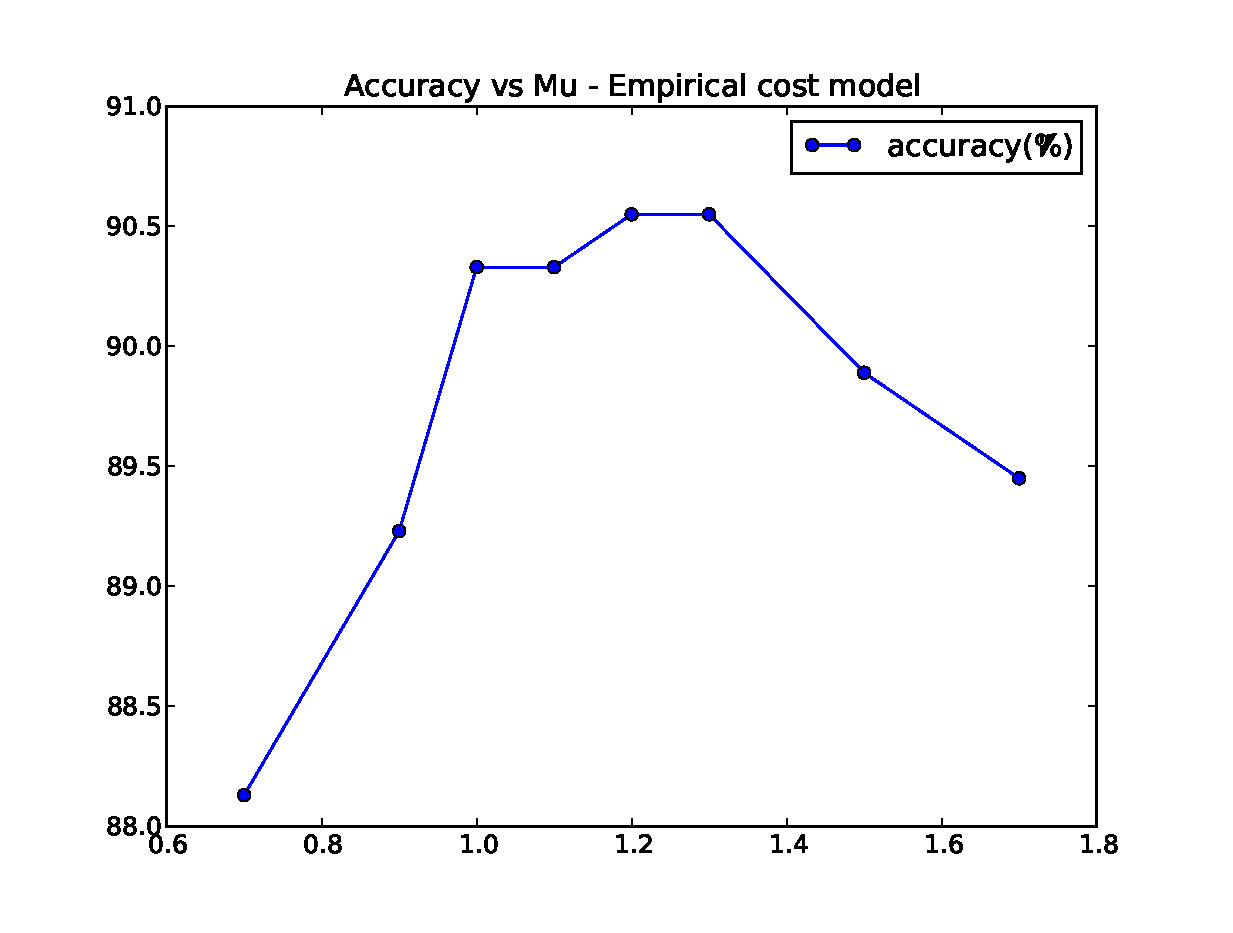
\includegraphics[width=0.9\linewidth]{mu}
\end{figure}

For uniform cost edit probability, the system is reluctant to perform an edit while the value is small, so you have small risk of wrongly modifying a correct query, but may not do correct modifications. As the value rises, there is a ``sweet spot" where accuracy peaks, and then accuracy plummets as the system is increasingly encouraged to make edits to fit the language model, often erroneously.

Also, we note that a query can only produce 5 types of outcomes, based on whether the input was correct in the first place, whether the spell corrector modified the query, and whether the output was correct. These statistics are important in understanding what kind of mistakes the corrector is making.
\begin{figure}[H]
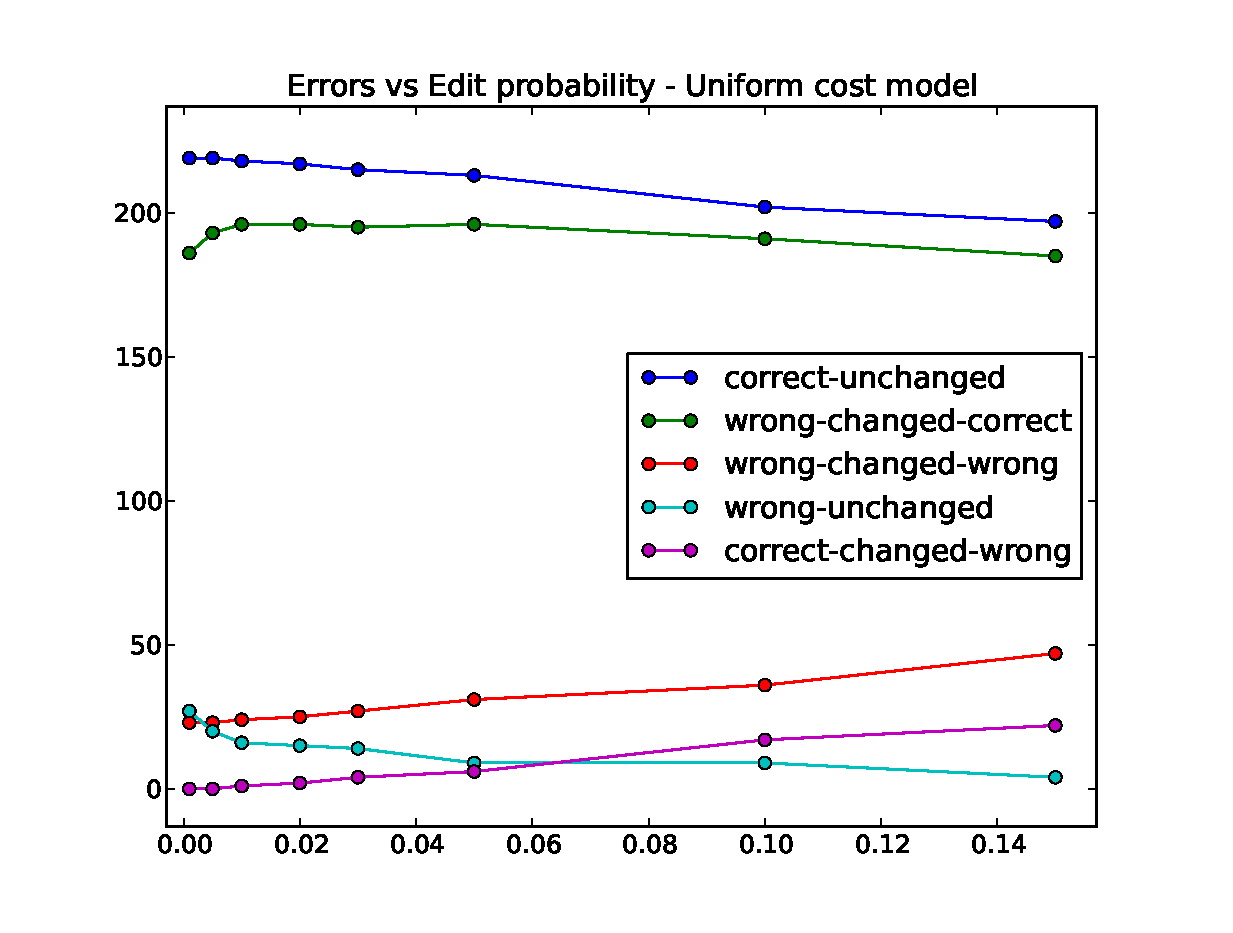
\includegraphics[width=0.9\linewidth]{editprob_err}
\end{figure}
As we study the above figure, the effect of edit probability on the uniform cost spell corrector is clear. When the edit probability is small, we never make the mistake of modifying a correct input query. As the probability is set higher, these kind of mistakes happen more and more often. On the other hand, with small edit probability, we fail to modify a large amount of incorrect queries. As the probability is set higher, many of these queries get modified.

\bibliographystyle{plain}
\bibliography{references}
\end{document}